%=========================================================

% Here you can choose to compile with or without solutions.
% However, this definition is ignored if you use any
% command from the `Makefile`.
\providecommand{\withSol}{\iftrue}

%=========================================================

\documentclass
[twoside,english,colorbacktitle,accentcolor=tud9c]
{tudexercise}

\usepackage[T1]{fontenc}
\usepackage[latin9]{inputenc}
\usepackage{amstext}
\usepackage{amsmath}
\usepackage{graphicx}
\usepackage{setspace}
\usepackage{multicol}
\usepackage{mathtools}
\usepackage{dsfont}
\usepackage{units}
\usepackage{subfigure}
\usepackage{color}
\usepackage{booktabs}
\usepackage{fancyref}
\usepackage[ngerman,english]{babel}
\usepackage{commath}

%=========================================================

\def\homework{1}
\def\homeworkVer{1}
\def\homeworkSolVer{1}
\def\lecture{Machine Learning}
\def\semester{Summer Semester 2018}
\def\prof{Prof. Dr. J. Peters, D. Tanneberg, B. Belousov}
\def\deadline{Due date: Wednesday, 02 May 2018 (before the lecture)}

%=========================================================

\ifcsname withSol\endcsname\else
  \expandafter\let\csname withSol\expandafter\endcsname
                  \csname iffalse\endcsname
\fi

\withSol
	\usepackage[solutions]{iasHomework}
\else
	\usepackage{iasHomework}
\fi

%=========================================================

% USE YOUR NAMES!
\newcommand{\studentdata}{}
%\newcommand{\studentdata}{John Doe, 1234567 \qquad Jane Doe, 7654321}

\begin{document}
	
	\hwtitle{}
	\maketitle
	
	\begin{examheader}
		\normalsize
		\vspace{-1em}
		Alessia, Di Blasi, ID Number \hfill \studentdata{}
		\vspace{-1em}
	\end{examheader} 
	
	\textbf{Name, Surname, ID Number \hfill \studentdata{}}

	\newif\ifvimbug
\vimbugfalse

\ifvimbug
\begin{document}
\fi

\exercise{Linear Algebra Refresher}
 

\begin{questions}

%----------------------------------------------

\begin{question}{Matrix Properties}{5}
A colleague of yours suggests matrix addition and multiplication are similar to scalars, thus commutative, distributive and associative properties can be applied.
Is the statement correct? Prove it analytically or give counterexamples (for both operations) considering three matrices $ A, B, C$ of size $n\times n$.

\begin{answer}
	\begin{itemize}
		\item Addition
			\begin{itemize}
				\item Commutative \\
				Given $ A = [ a_{ij} ]$ and $ B = [ b_{ij} ]$ $\forall i, j =  {1,2,...n}$, \\
				$A + B = [a_{ij} +b_{ij}] $, \\
				$B + A = [b_{ij} +a_{ij}] $. \\ 
				Since the sum of two scalars is commutative than the sum of two matrices is commutative.
				\item Associative
				Given $ A = [ a_{ij} ]$, $ B = [ b_{ij} ]$ and $ C = [ c_{ij} ]$ $\forall i, j =  {1,2,...n}$, \\
				$A + B + C = [ a_{ij} + b_{ij} + c_{ij} ]$ 
				$(A+B) + C = [ (a_{ij} + b_{ij}) + c_{ij} ]$
				Since the sum of two scalars is associative than the sum of two matrices is associative.
			\end{itemize}
		\item Multiplication
		 	\begin{itemize}
		 		\item Commutative \\
		 		This property is not verified. \\
		 		For instance, given \\
		 		\begin{equation*}
		 		A = ( \begin{array}{c c } 
		 		1 & 2  \\
		 		13& 4 \end{array} ),
		 		\end{equation*}
		 		\begin{equation*}
		 		B = ( \begin{array}{c c } 
		 		1 & 1  \\
		 		2& 3 \end{array} )
		 		\end{equation*}
		 		\begin{equation*}
		 		\Rightarrow 
		 		A*B = ( \begin{array}{c c } 
		 		5& 7  \\
		 		11& 15 \end{array} ) \ \&  \
		 		B*A = ( \begin{array}{c c } 
		 		4& 6  \\
		 		11& 16 \end{array} )
		 		\end{equation*}
		 		\item Distributive\\
		 		Given $ A = [ a_{ij} ]$, $ B = [ b_{ij} ]$ and $ C = [ c_{ij} ]$ $\forall i, j =  {1,2,...n}$. \\
		 		I have to prove that $ A*(B + C) = A*B + A*C $ \\
		 		$A*(B + C) =[ \sum_{k=1}^{n} a_{ik}*(b_{kj}+c_{kj}) =\sum_{k=1}^{n} a_{ik}b_{kj} + \sum_{k=1}^{n} a_{ik}c_{kj}]= A*B + A*C$\\
		 		\item Associative \\
		 		Given $ A = [ a_{ij} ]$, $ B = [ b_{ij} ]$ and $ C = [ c_{ij} ]$ $\forall i, j =  {1,2,...n}$, \\
		 		I have to prove that $(A*B)*C=A*(B*C)$. \\
		 		$(A*B)*C =[r_{ij}]$ where $r_{ij} = \sum_{k=1}^{n} (\sum_{l=1}^{n}a_{il}*b_{lk})c_{kj} =\sum_{k=1}^{n} \sum_{l=1}^{n}(a_{il}*b_{lk})*c_{kj} $ \\
		 		$A*(B*C) =[s_{ij}]$ where $s_{ij} = \sum_{k=1}^{n}a_{ik} (\sum_{l=1}^{n}b_{kl}*c_{lj}) = \sum_{k=1}^{n} \sum_{l=1}^{n}a_{il}*(b_{lk}*c_{kj})$.\\
		 			Since the multiplication of two scalars is associative than the multiplication of two matrices is associative.
		 	\end{itemize}
	\end{itemize}
\end{answer}

\end{question}

%----------------------------------------------

\begin{question}{Matrix Inversion}{6}
Given the following matrix 
\begin{equation*}
     A = ( \begin{array}{c c c} 
     1 & 2 & 3 \\
     1 & 2 & 4 \\
     1 & 4 & 5 \end{array} )
\end{equation*}
analytically compute its inverse $ A^{-1}$ and illustrate the steps.

If we change the matrix in
\begin{equation*}
     A = ( \begin{array}{c c c} 
     1 & 2 & 3 \\
     1 & 2 & 4 \\
     1 & 2 & 5 \end{array} )
\end{equation*}
is it still invertible? Why?

\begin{answer}
	\begin{enumerate}
		\item II - I and III - I\\
		\bigskip
		$	
		\left[\begin{array}{ccc|ccc}
			1 & 2 & 3 & 1&0&0    \\       
			1 & 2 & 4 & 0&1&0    \\       
			1 & 4 & 5 & 0&0&1     \\      
		\end{array} \right] =
		\left[\begin{array}{ccc|ccc}
		1 & 2 & 3 & 1&0&0    \\       
		0& 0 & 1 & -1&1&0    \\       
		0& 2 & 2 & -1&0&1     \\      
		\end{array} \right]
		$
		
		\item III divided by 2  and change of II with III \\
		\bigskip
		$	
		\left[\begin{array}{ccc|ccc}
		1 & 2 & 3 & 1&0&0    \\       
		0& 0 & 1 & -1&1&0    \\       
		0& 2 & 2 & -1&0&1     \\      
		\end{array} \right] =
		\left[\begin{array}{ccc|ccc}
		1 & 2 & 3 & 1&0&0    \\       
		0& 1 & 1 & -\frac{1}{2}&0&\frac{1}{2}    \\       
		0& 0 & 1 & -1&1&0     \\      
		\end{array} \right]
		$
		
		\item II - III and I - 3*III \\
		\bigskip
		$	
		\left[\begin{array}{ccc|ccc}
		1 & 2 & 3 & 1&0&0    \\       
		0& 1 & 1 & -\frac{1}{2}&0&\frac{1}{2}    \\       
		0& 0 & 1 & -1&1&0     \\      
		\end{array} \right] =
		\left[\begin{array}{ccc|ccc}
		1 & 2 & 0 & 4&-3&0    \\       
		0& 1 & 0 & \frac{1}{2}&-1&\frac{1}{2}    \\       
		0& 0 & 1 & -1&1&0     \\      
		\end{array} \right]
		$
		
		\item I- 2* II \\
		\bigskip
		$	
		\left[\begin{array}{ccc|ccc}
		1 & 2 & 0 & 4&-3&0    \\       
		0& 1 & 0 & \frac{1}{2}&-1&\frac{1}{2}    \\       
		0& 0 & 1 & -1&1&0     \\      
		\end{array} \right]=
		\left[\begin{array}{ccc|ccc}
		1 & 0 & 0 & 3&-1&-1    \\       
		0& 1 & 0 & \frac{1}{2}&-1&\frac{1}{2}    \\       
		0& 0 & 1 & -1&1&0     \\      
		\end{array} \right]
		$
	\end{enumerate}
 
 The second matrix is not invertible because the first and the second columns are linearly depends, so it is not a full rank matrix  so it is singular.
\end{answer}

\end{question}
	
%----------------------------------------------

\begin{question}{Matrix Pseudoinverse}{3}
	Write the definition of the right and left Moore-Penrose pseudoinverse of a generic matrix $A \in \R^{n\times m}$.
	
	Given $A \in \R^{2 \times 3}$, which one does exist? Write down the equation for computing it, specifying the dimensionality of the matrices in the intermediate steps.
	
\begin{answer}
\begin{itemize}
	\item Left Moore-Penrose pseudoinverse: \\
		$A^+ = (A^*A)^{-1}A^*$
	\item Right Moore-Penrose pseudoinverse: \\
		$A^+ = A^*(A^*A)^{-1}$
\end{itemize}
\end{answer}
\end{question}

%----------------------------------------------

\begin{question}{Eigenvectors \& Eigenvalues}{6}
What are eigenvectors and eigenvalues of a matrix $A$? Briefly explain why they are important in Machine Learning.

\begin{answer}\end{answer}

\end{question}

%----------------------------------------------

\end{questions}

	
	\newif\ifvimbug
\vimbugfalse

\ifvimbug
\begin{document}
\fi

\exercise{Statistics Refresher}
 

\begin{questions}

%----------------------------------------------

\begin{question}{Expectation and Variance}{8}
Let $\Omega$ be a finite set and $P:\Omega\rightarrow\R$ a probability measure that (by definition) satisfies $P(\omega)\geq0$ for all $\omega\in\Omega$ and $\sum_{\omega\in\Omega}P(\omega)=1$. 
Let $f:\Omega\rightarrow\R$ be an arbitrary function on $\Omega$.

\textbf{1)} Write the definition of expectation and variance of $f$ and discuss if they are linear operators.

\textbf{2)} You are given a set of three dices $\{A,B,C\}$.
The following table describes the outcome of six rollouts for these dices, where each column shows the outcome of the respective dice. 
(Note: assume the dices are standard six-sided dices with values between 1-6)
\begin{equation*}
\begin{array}{r|cccccc}
    A & 4 & 4 & 2 & 4 & 1 & 1 \\
    \hline
    B & 3 & 6 & 3 & 3 & 4 & 3 \\
    \hline
    C & 5 & 5 & 2 & 1 & 1 & 1 
\end{array}
\end{equation*}
Estimate the expectation and the variance for each dice using unbiased estimators. (Show your computations).

\textbf{3)} According to the data, which of them is the ``most rigged''? Why?

\begin{answer}
\textbf{1)} Expected value is defined as:
$$E(f) = \sum_{\omega \in \Omega} f(\omega)P(\omega)$$
Variance is defined as:
$$var(f) = \sum_{\omega \in \Omega} (f(\omega)-E(f))^2P(\omega)$$

$ E[\alpha f(x) + \beta g(x)] = \alpha  E[f(x)] + \beta E[g(x)]$ thanks to the Expectation operator properties. So it is a linear operator. \\
$ Var[\alpha f(x) + \beta g(x)] = \alpha^{2}  Var[f(x)] + \beta^{2} E[g(x)] + 2\alpha \beta Cov[f(x),g(x)] $. So it is not a linear operator \\ \\
\textbf{2)} \begin{itemize}
	\item \textbf{Dice A: } \newline
	$$
	E(A) = \frac{1}{6} (4+4+2+4+1+1 ) = \frac{16}{6}
	$$
	
	$$
	var(A) = \frac{3}{5}(4-\frac{16}{6})^2 + \frac{1}{5}(2-\frac{16}{6})^2 + \frac{2}{5}(1-\frac{16}{6})^2 = \frac{34}{15}
	$$
	
	\item \textbf{Dice B: } \newline
	$$
	E(A) = \frac{1}{6} (3+6+3+3+4+3) = \frac{11}{3}
	$$
	
	$$
	var(A) = \frac{4}{5}(3-\frac{11}{3})^2 + 
	\frac{1}{5}(6-\frac{11}{3})^2 + 
	\frac{1}{5}(4-\frac{11}{3})^2 = \frac{22}{15}
	$$
	
	\item \textbf{Dice C: } \newline
	$$
	E(A) = \frac{1}{6} (5+5+2+1+1+1) = \frac{5}{2}
	$$
	
	$$
	var(A) = \frac{2}{5}(5-\frac{5}{2})^2 + 
	\frac{1}{5}(2-\frac{5}{2})^2 + 
	\frac{3}{5}(1-\frac{5}{2})^2 = \frac{39}{10}
	$$
\end{itemize}

\textbf{3)}
The most rigged dice is the dice with higher observed standard deviation of the result frequencies with respect to the one of a balanced dice.\\
A balanced dice is expected to output any number with probability $1/6$.
\begin{itemize}
	\item \textbf{A} 
	$$
	\sqrt{
		(\frac{2}{6}-\frac{1}{6})^2 +
		(\frac{1}{6}-\frac{1}{6})^2 +
		(\frac{0}{6}-\frac{1}{6})^2 +
		(\frac{3}{6}-\frac{1}{6})^2 +
		(\frac{0}{6}-\frac{1}{6})^2 +
		(\frac{0}{6}-\frac{1}{6})^2
	} = 
	$$
	$$
	= \sqrt{\frac{2}{9}} = \frac{\sqrt{2}}{3} \approx 0.4714
	$$
	\item \textbf{B} 
	$$
	\sqrt{
		(\frac{0}{6}-\frac{1}{6})^2 +
		(\frac{0}{6}-\frac{1}{6})^2 +
		(\frac{4}{6}-\frac{1}{6})^2 +
		(\frac{1}{6}-\frac{1}{6})^2 +
		(\frac{0}{6}-\frac{1}{6})^2 +
		(\frac{1}{6}-\frac{1}{6})^2
	} = 
	$$
	$$
	= \sqrt{\frac{1}{3}} = \frac{1}{\sqrt{3}} \approx 0.5774
	$$
	
	
	\item \textbf{C} 
	$$
	\sqrt{
		(\frac{3}{6}-\frac{1}{6})^2 +
		(\frac{1}{6}-\frac{1}{6})^2 +
		(\frac{0}{6}-\frac{1}{6})^2 +
		(\frac{0}{6}-\frac{1}{6})^2 +
		(\frac{2}{6}-\frac{1}{6})^2 +
		(\frac{0}{6}-\frac{1}{6})^2
	} = 
	$$
	$$
	= \sqrt{\frac{2}{9}} = \frac{\sqrt{2}}{3} \approx 0.4714
	$$
\end{itemize}

Hence the dice $B$ is the most rigged since he has the biggest standard deviation.
\end{answer}

\end{question}

%----------------------------------------------

\begin{question}{It is a Cold World}{7}
Consider the following three statements:
\\
a) A person with a cold has backpain $25\%$ of the time.
\\
b) $4\%$ of the world population has a cold.
\\
c) $15\%$ of those who do not have a cold, still have backpain.

\textbf{1)} Identify random variables from the statements above and define a unique symbol for each of them.\\
\textbf{2)} Define the domain of each random variable.\\
\textbf{3)} Represent the three statements above with your random variables.\\
\textbf{4)} If you suffer from backpain, what are the chances that you suffer from a cold? (Show all the intermediate steps.)

\begin{answer}
	\textbf{1)} Let $C$ be a Bernoulli random variable that identify if a person has or not cold. \\
	Let $B$ be a Bernoulli random variable that identify if a person has or not backpain. \\
	\textbf{2)} The domain of bot $C$ and $B$ is $\{0, 1\}$ since they are Bernoulli.\\
	\textbf{3)} 
	\begin{itemize}
	\item [a)] $ P( B=1 | C=1 ) = 25\% $
	\item [b)] $ P( C=1 ) = 4\% $
	\item [c)] $ P( B=1 | C=0 ) = 15\% $
\end{itemize}
	\textbf{4)} We want to obtain the following probability: $ P( C=1 | B=1 ) $ \\
	Applying Bayes theorem:
	$$
	P( C=1 | B=1 ) = \frac{P( B=1 | C=1 ) P( C=1 )}{P( B=1 )}
	$$
	Both $ P( B=1 | C=1 ) $ and $ P( C=1 ) $ are known. \\
	Now we need to calculate only $P(B=1)$:
	$$
	P(B=1) = P( B=1 | C=1 ) \cdot P( C=1 ) + P( B=1 | C=0 ) \cdot P( C=0 ) =
	$$
	$$
	= \frac{25}{100} \cdot \frac{4}{100} + \frac{15}{100} \cdot \frac{96}{100} = 0.154
	$$
	Hence:
	$$
	P( C=1 | B=1 ) = \frac{P( B=1 | C=1 ) P( C=1 )}{P( B=1 )} = \frac{0.25 \cdot 0.04}{0.154} = \frac{5}{77}
	$$
\end{answer}

\end{question}


%----------------------------------------------

\begin{question}{Journey to THX1138}{10}
	After the success of the \href{http://rosetta.esa.int/}{Rosetta mission}, ESA decided to send a spaceship to rendezvous with the comet THX1138. 
	This spacecraft consists of four independent subsystems $A,B,C,D$. 
	Each subsystem has a probability of failing during the journey equal to $1/3$. 
	\\
	1) What is the probability of the spacecraft $S$ to be in working condition (i.e., all subsystems are operational at the same time) at the rendezvous?
	\\
	2) Given that the spacecraft $S$ is not operating properly, compute	analytically the probability that \textbf{only} subsystem $A$ has failed. 
	\\
	3) Instead of computing the probability analytically, do a simple simulation experiment and compare the result to the previous solution. 
	Include a snippet of your code. 
	\\
	4) An improved spacecraft version has been designed.
	The new spacecraft fails if the critical subsystem $A$ fails, or any two subsystems of the remaining $B,C,D$ fail. 
	What is the probability that \textbf{only} subsystem $A$ has failed, given that the spacecraft $S$ is failing? 
	
	
\begin{answer}
	1)Since the random variables $A$, $B$, $C$, $D$ are i.i.d. the probability of the disjunction is obtained simply by multiplying the single probabilities, hence:
	$$
	P(A=1 \cap B=1 \cap C=1 \cap D=1) = P(A=1) \cdot P(B=1) \cdot P(C=1) \cdot P(D=1) = (\frac{2}{3})^4
	$$\\
	2)$$
	P(A=0 \cap B,C,D = 1 \ | \ S = 0) = \frac{P(S=0 | A= 0 \cap B=1 \cap C=1 \cap D=1) \cdot P(A=1 \cap B=1 \cap C=1 \cap D=1)}{P(S=0)} = 
	$$ \\
	$$
	 = \frac{1 \cdot (\frac{2}{3})^3 \cdot \frac{1}{3}}{1- (\frac{2}{3})^4} = \frac{8}{65}
	$$\\
	3)
\lstinputlisting[language=Python]{rosetta.py}	
%	\begin{lstlisting}
%		TRIES = 10000000
%		PROB = 2. / 3
%		a = np.random.binomial(1, PROB, TRIES)
%		b = np.random.binomial(1, PROB, TRIES)
%		c = np.random.binomial(1, PROB, TRIES)
%		d = np.random.binomial(1, PROB, TRIES)
%		success = 0
%		for i in range(TRIES):
%		if a[i] == 0 and b[i] == 1 and c[i] == 1 and d[i] == 1:
%		success += 1
%		print (success / TRIES)
%	\end{lstlisting}
		
	
	The analytical result is $8/81 \approx 0.09876543209$\\
	The result of the simple simulation above (in one specific computation) was $0.0986829$, and they match up to the fourth decimal digit.

	4) We know that 
	$$
	P(S=0) \ = \ P(S=0 \  | \ A=1) \cdot P(A=1) + P(S=0 \ | \ A=0) \cdot P(A=0) \ = \  ( {{3}\choose{2}} \frac{2}{3} (\frac{1}{3})^2 + (\frac{1}{3})^3) \cdot \frac{2}{3} + 1 \cdot  \frac{1}{3}=\frac{41}{81}
	$$\\
	Hence 
	$$
	P(A=0 \cap B=1 \cap C=1 \cap D=1 \ | \ S=0) \ = $$$$ = \frac{P(S=0 \  | \ A=0 \cap  B=1 \cap C=1 \cap D=1) \cdot P( \ A=0 \cap  B=1 \cap C=1 \cap D=1) }{P(S = 0)}  = 
	$$$$
	= \frac{1 \cdot \frac{1}{3} \cdot (\frac{2}{3})^3}{\frac{41}{81}} = \frac{8}{41}  \approx 0.19512
	$$
\end{answer}
	
\end{question}


\end{questions}

	
	\newif\ifvimbug
\vimbugfalse

\ifvimbug
\begin{document}

\end{document}
\fi

\exercise{Optimization and Information Theory}
 

\begin{questions}

%----------------------------------------------


\begin{question}{Entropy}{5}
You work for a telecommunication company that uses a system to transmit four different symbols ${S_1, S_2, S_3, S_4}$ through time. 
In the current system, each symbol has a probability to occur according to the following table 
\begin{equation*}
\begin{array}{c|c|c|c|c}
 & S_1 & S_2 & S_3 & S_4 \\
\hline
p_i & 0.03    & 0.62    & 0.26    & 0.09
\end{array}
\end{equation*}
Compute the entropy of the system and write the minimum number of bits requires for transmission.

\begin{answer}
$ H(p) = - \sum_{i=1}^{4}p_i \cdot log_2 p_i = 1.397298 $ \\
Minimum number of bits = $log_2 4$ = 2
\end{answer}

\end{question}

%----------------------------------------------

\begin{question}{Constrained Optimization}{25}
After an upgrade of the system, your boss asks you to change the probabilities of transmission in order to maximize the entropy. However, the new system has the following constraint
\begin{equation*}
    4 = \sum_{i=1}^4 2p_i i.
\end{equation*}
\textbf{1)} Formulate it as a constrained optimization problem. Do you need to include additional constrains beside the one above?
\\
\textbf{2)} Write down the Lagrangian of the problem. Use one Lagrangian multiplier per constraint.
\\
\textbf{3)} Compute the partial derivatives of the Lagrangian above for each multiplier and the objective variable. Is it easy to solve it analytically? 
\\
\textbf{4)} Formulate the dual function of this constrained optimization problem. Solve it analytically.
\\
\textbf{5)} Name one technique for numerically solve these problems and briefly describe it.

\begin{answer}
\textbf{1)}
$ \max\limits_{p} \ J(p) = - \sum\limits_{i=1}^{4}p_i\log_2 p_{i} $\\
s.t.
\begin{math}
\begin{cases}
 f_{1}(p) = \sum\limits_{i=1}^{4} p_{i}i  -2=0 \\f_{2}(p) = \sum\limits_{i=1}^{4} p_{i} -1= 0
\end{cases}
\end{math}\\
\textbf{2)}
\begin{math}
L(p,\lambda) = -\sum\limits_{i=1}^{4} p_{i} \log_2 p_{i}+\lambda_{1}(p_{1}+2p_{2}+3p_{3}+4p_{4}-2)+\lambda_{2}(p_{1}+p_{2}+p_{3}+p_{4}-1) 
\end{math}
\\
\textbf{3)} 
$ \frac{\partial L}{\partial p_{1}} = -\log_2 p_1 - \log_2 e + \lambda_{1} + \lambda_{2} $ \\ \\
$ \frac{\partial L}{\partial p_{2}} = -\log_2 p_2 - \log_2 e + 2 \lambda_{1} + \lambda_{2} $ \\ \\ 
$ \frac{\partial L}{\partial p_{3}} = -\log_2 p_3 - \log_2 e + 3 \lambda_{1} + \lambda_{2} $ \\ \\
$ \frac{\partial L}{\partial p_{4}} =-\log_2 p_4 - \log_2 e + 4 \lambda_{1} + \lambda_{2} $ \\ \\
$ \frac{\partial L}{\partial \lambda_{1}} = p_{1} + 2 p_{2} + 3 p_{3} + 4 p_{4} - 2  $ \\ \\
$ \frac{\partial L}{\partial \lambda_{2}} = p_{1} + p_{2} + p_{3} + p_{4} - 1 $ \\ \\
It is NOT easy to solve it analytically. \\ \\
\textbf{4)} 
Let the derivatives be equal to 0, we are able to write $p_i $ depending on $\lambda_{1}$ and $\lambda_{2}$
$ \frac{\partial L}{\partial p_{1}} = 0 \Rightarrow p_{1}=\frac{1}{e}2^{\lambda_{1}+\lambda_{2}}$ \\ \\
$ \frac{\partial L}{\partial p_{2}} = 0 \Rightarrow p_{2}=\frac{1}{e}2^{2 \lambda_{1}+\lambda_{2}} $ \\ \\ 
$ \frac{\partial L}{\partial p_{3}} = 0 \Rightarrow p_{3}=\frac{1}{e}2^{3 \lambda_{1}+\lambda_{2}}  $ \\ \\
$ \frac{\partial L}{\partial p_{4}} = 0 \Rightarrow p_{4}=\frac{1}{e}2^{4 \lambda_{1}+\lambda_{2}} $ \\ \\
Then: \\
$  L(\theta,\lambda) = - \frac{1}{e}2^{\lambda_{1}+\lambda_{2}} \log_2(\frac{1}{e}2^{\lambda_{1}+\lambda_{2}}) - \frac{1}{e}2^{2 \lambda_{1}+\lambda_{2}} \log_2(\frac{1}{e}2^{2 \lambda_{1}+\lambda_{2}})
- \frac{1}{e}2^{3 \lambda_{1}+\lambda_{2}} \log_2(\frac{1}{e}2^{3 \lambda_{1}+\lambda_{2}}) - \frac{1}{e}2^{4 \lambda_{1}+\lambda_{2}} \log_2(\frac{1}{e}2^{4 \lambda_{1}+\lambda_{2}}) + \\
\lambda_{1} (\frac{1}{e}2^{\lambda_{1}+\lambda_{2}} + \frac{1}{e} 2 \cdot 2^{2 \lambda_{1}+\lambda_{2}} + \frac{1}{e} 3 \cdot 2^{3 \lambda_{1}+\lambda_{2}} + \frac{1}{e} 4 \cdot 2^{4 \lambda_{1}+\lambda_{2}} - 2) 
+ \lambda_{2} (\frac{1}{e}2^{\lambda_{1}+\lambda_{2}} + \frac{1}{e} 2^{2 \lambda_{1}+\lambda_{2}} + \frac{1}{e} 2^{3 \lambda_{1}+\lambda_{2}} + \frac{1}{e} 2^{4 \lambda_{1}+\lambda_{2}} - 1) = \\ \\
= - \frac{1}{e}2^{\lambda_{1}+\lambda_{2}} \left[\log_2 \frac{1}{e} + \lambda_{1} + \lambda_{2} - \lambda_{1} - \lambda_{2} \right] 
- \frac{1}{e}2^{2 \lambda_{1}+\lambda_{2}} \left[\log_2 \frac{1}{e} + 2 \lambda_{1} + \lambda_{2} - 2 \lambda_{1} - \lambda_{2} \right] +\\ \\
- \frac{1}{e}2^{3 \lambda_{1}+\lambda_{2}} \left[\log_2 \frac{1}{e} + 3 \lambda_{1} + \lambda_{2} - 3 \lambda_{1} - \lambda_{2} \right] 
- \frac{1}{e}2^{4 \lambda_{1}+\lambda_{2}} \left[\log_2 \frac{1}{e} + 4 \lambda_{1} + \lambda_{2} - 4 \lambda_{1} - \lambda_{2} \right] -2 \lambda_{1} - \lambda_{2} = \\ \\ \\
= \frac{1}{e} log_2^{e} 2^{\lambda_{2}} \left[2^{\lambda_{1}} + 2^{2 \lambda_{1}} + 2^{3 \lambda_{1}} + 2^{4 \lambda_{1}} \right] - 2 \lambda_{1} - \lambda_{2} \\ \\ $

$ \frac{\partial L}{\partial \lambda_{1}} = \frac{log_2^{e}}{e} 2^{\lambda_{2}} \left[2^{\lambda_{1}} \ln(2) + 2 \cdot 2^{2 \lambda_{1}} \ln(2) + 3 \cdot 2^{3 \lambda_{1}} \ln(2) + 4 \cdot 2^{4 \lambda_{1}} \ln(2)\right] - 2  $ \\ \\
$ \frac{\partial L}{\partial \lambda_{2}} = \frac{log_2^{e}}{e} 2^{\lambda_{2}} \ln(2) \left[2^{\lambda_{1}} + 2^{2 \lambda_{1}} + 2^{3 \lambda_{1}} + 2^{4 \lambda_{1}} \right] - 1  $

Letting the two derivatives be equal to 0, we obtain the following system:
\begin{equation}
\begin{cases}
\frac{1}{e} 2^{\lambda_{2}} \left[2^{\lambda_{1}} + 2 \cdot 2^{2 \lambda_{1}} + 3 \cdot 2^{3 \lambda_{1}} + 4 \cdot 2^{4 \lambda_{1}} \right] = 2\\ 
\frac{1}{e} 2^{\lambda_{2}} \left[2^{\lambda_{1}} + 2^{2 \lambda_{1}} + 2^{3 \lambda_{1}} + 2^{4 \lambda_{1}} \right] = 1
\end{cases}
\end{equation}

Dividing the first equation by the second one and letting $x=2^{\lambda_{1}}$, we obtain: \\ \\
$ \frac{x+2x^{2}+3x^{3}+4x^{4}}{x+x^{2}+x^{3}+x^{4}}=2 \Rightarrow \frac{1+2x+3x^{2}+4x^{3}}{1+x+x^{2}+x^{3}}=2 
\Rightarrow 2x^{3}+x^{2}-1=0 \Rightarrow x \approx 0.6573  \Rightarrow 2^{\lambda_{1}} \approx 0.6573 \Rightarrow \lambda_{1} = -0.6054 $ \\ \\
$ 2^{\lambda_{2}} = e \frac{1}{2^{\lambda_{1}}+ 2^{2 \lambda_{1}} + 2^{3 \lambda_{1}} + 2^{4 \lambda_{1}}} \approx 1.7425 \Rightarrow \lambda_{2} \approx 0.8012 $ \\ \\
$ p_{1}=\frac{1}{e}(0.6573)(1.7425)=0.4213 $ \\ \\
$ p_{2}=\frac{1}{e}(0.6573)^{2}(1.7425)=0.277 $ \\ \\
$ p_{3}=\frac{1}{e}(0.6573)^{3}(1.7425)=0.182 $ \\ \\
$ p_{4}=\frac{1}{e}(0.6573)^{4}(1.7425)=0.12 $ \\

\textbf{5)} We can use the steepest descent method: it is a first-order iterative optimization algorithm for finding a local minimum of a function. It uses  steps that are proportional to the opposite of the gradient of the function at the current point. However if steps are proportional to the gradient, the method returns a local maximum of that function (gradient ascent).
\end{answer}

\end{question}
	

%----------------------------------------------

\begin{question}{Numerical Optimization}{10}
Rosenbrock's function (to be minimized) is defined as 
$$f(\boldsymbol{x}) = \sum_{i=1}^{n-1} \left[ 100 (x_{i+1} - x_{i}^{2})^{2} + (x_{i} - 1)^{2}\right].$$
Write in Python a simple gradient descent algorithm and simulate it for 10,000 steps on Rosenbrock's function with $n=20$. Attach a snippet of your algorithm, discuss the effects of the learning rate and attach a plot of your learning curve with your best learning rate.

\begin{answer}
\lstinputlisting[language=Python]{Rosembrock.py}
\medskip \medskip
The learning rate determines how fast or slow the algorithm will move towards the optimal weights. If the learning rate is very large the algorithm will skip the optimal solution. If it is too small the algorithm will need too many iterations to converge to the best values.
In this case the best learning rate is $ 10^{-6} $. The plot rapresents the parameters curve that tend to the minimum value. \\
\begin{center}
	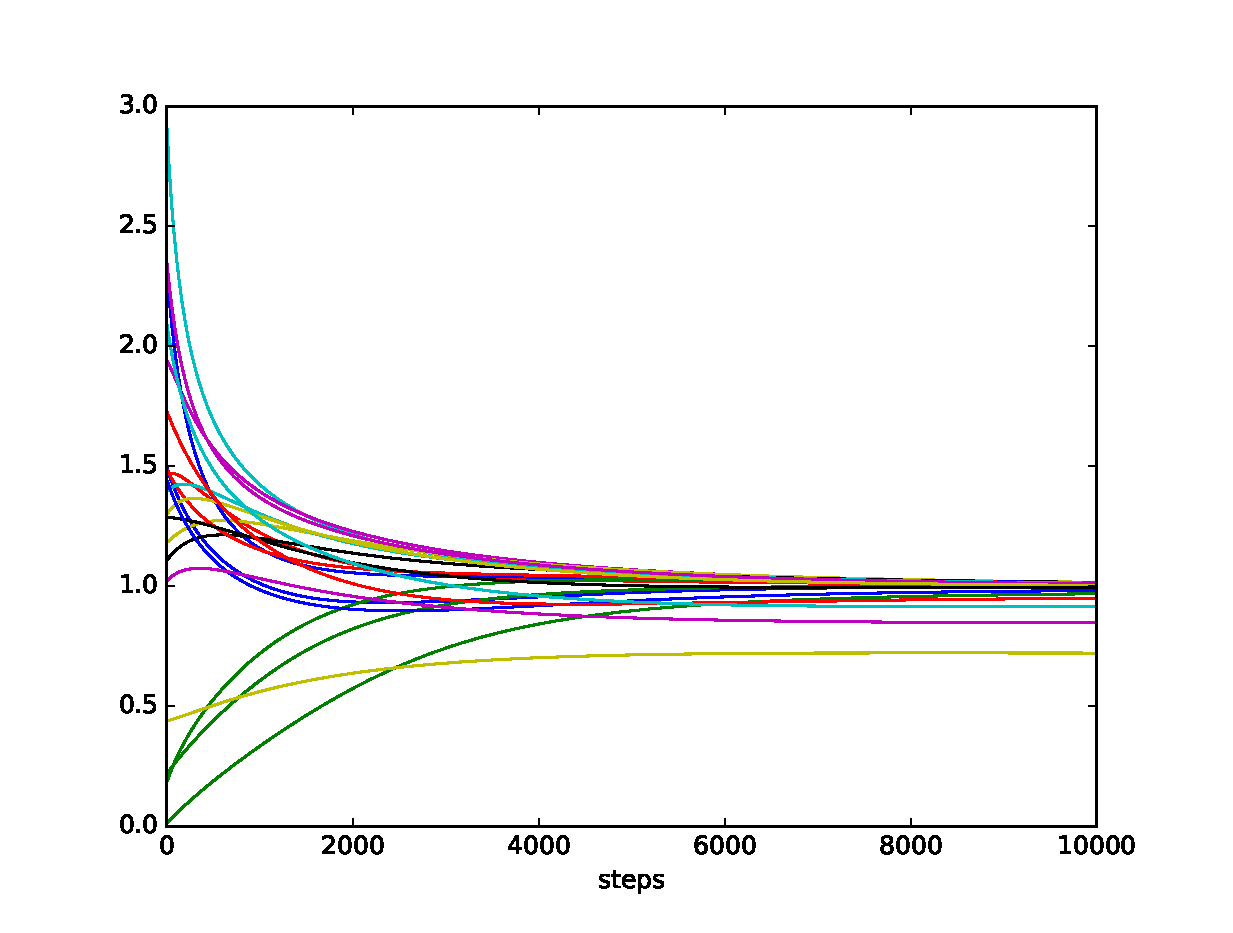
\includegraphics [scale=0.75]{rosembrockPlot.eps}
\end{center}

\end{answer}

\end{question}

%----------------------------------------------

\begin{question}[bonus]{Natural Gradient}{10}
Let $\theta \in \mathbb{R}^n$ be a parameter vector
and $J \colon \mathbb{R}^n \to \mathbb{R}$ a cost function.
The negative gradient $-\nabla J(\theta)$ is sometimes called
the \emph{steepest descent direction}. But is it really?
To be able to claim that it is \emph{the} steepest descent direction,
we should compare it to other descent directions
and pinpoint what is so unique about the negative gradient direction.

\textbf{Covariant gradient.}
A fair way to compare descent directions is to make
a small step of fixed length, say $\varepsilon$,
in every direction~$\Delta \theta$ and check
which direction leads to the greatest decrease in $J(\theta)$.
Since we assume that the step size is small, we can evaluate
the decrease in $J(\theta)$ using its first-order Taylor approximation
\begin{equation*}
  J(\theta + \Delta \theta) - J(\theta) \approx
  \nabla J(\theta)^T \Delta \theta.
\end{equation*}
To make precise what we mean by `small' step size,
we need to introduce a norm (or a distance)
in the space of parameters $\theta$.
A good choice, that among other advantages captures the intuition
that some parameters may influence the objective function more
than others,
is the generic quadratic norm
\begin{equation*}
  \norm{\Delta \theta}^2 =
  \frac{1}{2}\Delta \theta^T F(\theta) \Delta \theta
\end{equation*}
with a positive-definite matrix $F(\theta)$;
note that in general $F$ may depend on $\theta$.

\textbf{1)} Find the direction $\Delta \theta$ that yields
the largest decrease in the linear approximation of $J(\theta)$
for a fixed step size~$\varepsilon$.
Does this direction coincide with $-\nabla J(\theta)$?
The direction that you found is known as the
negative covariant gradient direction.

\textbf{Natural gradient.}
In statistical models, parameter vector $\theta$ often
contains parameters of a probability density function $p(x; \theta)$
(for example, mean and covariance of a Gaussian density);
thus, the cost function $J$ depends on~$\theta$ indirectly
through $p(x; \theta)$.
This two-level structure gives a strong hint as to what matrix $F$
to pick for measuring the distance in the parameter space
in the most `natural' way.
Namely, one can carry over the notion of `distance' between
probability distributions $p(x; \theta + \Delta \theta)$
and $p(x; \theta)$ (which is known from information theory
to be well captured by the Kullback-Leibler divergence)
to the distance between the corresponding parameter vectors
$\theta + \Delta \theta$ and $\theta$.

\textbf{2)} Obtain the quadratic Taylor approximation
of the KL divergence
from $p(x; \theta)$ to $p(x; \theta + \Delta \theta)$ in the form
\begin{equation*}
  KL(p(x; \theta + \Delta \theta) || p(x; \theta)) \approx
  \frac{1}{2}\Delta \theta^T F(\theta) \Delta \theta.
\end{equation*}
Covariant gradient with the matrix $F(\theta)$ that you found
is known as the natural gradient.

\begin{answer}
\textbf{1)} $ \underset{\Delta \theta}{\operatorname{argmin}} \ \nabla J(\theta)^{T}\Delta \theta $ \ \ \ \ s.t. $ \frac{1}{2}\Delta \theta^{T}F(\theta)\Delta \theta=\epsilon^{2} $. \\
Let $ F(\theta)=\epsilon^{2} D^{T}D $ and $ z=D\Delta \theta $ \\ \\
$ \underset{\Delta \theta}{\operatorname{argmin}} \ \Delta \theta^{T} \nabla J(\theta) $ \ \ \ \ s.t. $ z^{T}z=1 $ \\ \\
$ D^{-1} \ \underset{z}{\operatorname{argmin}} (D^{-1}z)^{T}\nabla J(\theta) $ \ \ \ \ s.t. $ z^{T}z=1 $ \\ \\
$ D^{-1} \ \underset{z}{\operatorname{argmin}} \ z^{T}D^{-T}\nabla J(\theta) $ \ \ \ \ s.t. $ z^{T}z=1 $ \\ \\
$ \propto D^{-1}[-D^{-T}\nabla J(\theta)]\propto - F(\theta)^{-1}\nabla J(\theta) $ \\ \\

\textbf{2)} We know that: \\ \\
$ \log \frac{P(x;\theta + \Delta \theta)}{P(x;\theta)} = \log P(x;\theta + \Delta \theta) - \log P(x;\theta) \approx 
\frac{\partial}{\partial \theta} \log P(x;\theta)^{T} \Delta \theta + \frac{1}{2} \Delta \theta^{T} \frac{\partial^{2}}{\partial \theta^{2}} \log  P(x;\theta)\Delta \theta $. \\ \\
Hence: \\
$ D_{KL}(P(x;\theta + \Delta \theta) || P(x;\theta)) = \sum \limits_{x} P(x;\theta + \Delta \theta) \log \frac{P(x;\theta + \Delta \theta)}{P(x;\theta)} $ \\ \\
$ \simeq \sum \limits_{x} [P(x;\theta) + \frac{\partial}{\partial \theta} P(x;\theta)^{T} \Delta \theta + \frac{1}{2}\Delta \theta^{T} \frac{\partial^{2}}{\partial \theta^{2}} P(x;\theta)\Delta \theta] \cdot [\frac{\partial}{\partial \theta} \log P(x;\theta)^{T}\Delta \theta + \frac{1}{2} \Delta \theta^{T} \frac{\partial^{2}}{\partial \theta^{2}} \log P(x;\theta)\Delta \theta] $ \\ \\
$ \simeq \sum \limits_{x} \left[P(x;\theta) (\frac{\frac{\partial}{\partial \theta} P(x;\theta)}{P(x;\theta)})^{T}\Delta \theta + \frac{1}{2}\Delta \theta^{T}P(x;\theta) \cdot
\frac{P(x;\theta) \frac{\partial^{2} P(x;\theta)}{\partial \theta^{2}} - (\frac{\partial P(x;\theta)}{\partial \theta})^{T}(\frac{\partial P(x;\theta)}{\partial \theta})}{P^{2}(x;\theta)} \cdot \Delta \theta \right ] + \\ \\
+ \sum \limits_{x}\Delta \theta^{T} (\frac{\partial}{\partial \theta} P(x;\theta)) (\frac{\frac{\partial}{\partial \theta} P(x;\theta)}{P(x;\theta)})^{T} \Delta \theta $ \\ \\

$ = \sum \limits_{x} \left[ (\frac{\partial}{\partial \theta} P(x;\theta))^{T}\Delta \theta + \frac{1}{2}\Delta \theta^{T}(
 \frac{\partial^{2} P(x;\theta)}{\partial \theta^{2}} -P(x;\theta)(\frac{\frac{\partial P(x;\theta)}{\partial \theta}}{P(x;\theta)})^{T}(\frac{\frac{\partial P(x;\theta)}{\partial \theta}}{P(x;\theta)})) \cdot \Delta \theta \right ]  \\ \\
+ \sum \limits_{x}\Delta \theta^{T} (\frac{\partial}{\partial \theta} P(x;\theta)) (\frac{\frac{\partial}{\partial \theta} P(x;\theta)}{P(x;\theta)})^{T} \Delta \theta $ \\ \\

$ = (\frac{\partial}{\partial \theta} \sum \limits_{x}P(x;\theta))^{T} \Delta \theta + \frac{1}{2} \Delta \theta^{T} (\frac{\partial^{2}}{\partial \theta^{2}}\sum \limits_{x}P(x;\theta)) \Delta \theta + 
\frac{1}{2} \Delta \theta^{T} (\sum \limits_{x} P(x;\theta) (\frac{\partial}{\partial \theta} \log P(x;\theta))(\frac{\partial}{\partial \theta} \log P(x;\theta))^{T})\Delta \theta $ \\ \\ 
$ = (\frac{\partial}{\partial \theta} 1)^{T} \Delta \theta + \frac{1}{2} \Delta \theta^{T} (\frac{\partial^{2}}{\partial \theta^{2}}1) \Delta \theta + 
\frac{1}{2} \Delta \theta^{T} (\sum \limits_{x} P(x;\theta) (\frac{\partial}{\partial \theta} \log P(x;\theta))(\frac{\partial}{\partial \theta} \log P(x;\theta))^{T})\Delta \theta $ \\ \\ 
$ = \frac{1}{2} \Delta \theta^{T}F(\theta)\Delta \theta $
\end{answer}

\end{question}

%----------------------------------------------

\begin{question}[bonus]{Gradient Descent Variants}{5}
Throughout this class we have seen that gradient descent is one of the most used optimization techniques in Machine Learning. This question asks you to deepen the topic by conducting some research by yourself.

\textbf{1)} There are several variants of gradient descent, namely \emph{batch, stochastic} and \emph{mini-batch}. Each variant differs in how much data we use to compute the gradient of the objective function. 
Discuss the differences among them, pointing out pros and cons of each one.

\textbf{2)} Many gradient descent optimization algorithms use the so-called \emph{momentum} to improve convergence. What is it? Is it always useful?

\begin{answer}
\textbf{1)} In Gradient Descent methods, parameters have to be updated according to the following formula: \\ $\theta=\theta + \alpha \nabla J(\theta)$.	\\
Suppose we have data ${(x_i,y_i)}, \\ i=1:M$
\begin{itemize}
	\item Batch GD: All data are used to compute the approzimation of $\nabla J(\theta)$: \\
	$\nabla J(\theta) = \frac{1}{M}\sum \limits _{i=1}^M(\widehat{y_i}-y_i)x_i$
	\item Stochastic GD: Only a sample is used to compute the approzimation of $\nabla J(\theta)$:\\
	$\nabla J(\theta) =(\widehat{y_i}-y_i)x_i$
	\item Mini-batch GD: Only N data are used to compute the approzimation of $\nabla J(\theta)$:\\
	$\nabla J(\theta) = \frac{1}{N}\sum \limits _{i=1}^N(\widehat{y_i}-y_i)x_i$
\end{itemize}
Batch (and Mini-Batch) gradient descent is more computationally efficient than stochastic gradient descent and it has a more stable error gradient. However The more stable error gradient may result in premature convergence of the model to a less optimal set of parameters.\\
\textbf{2)} Momentum takes into account the update $\Delta \theta$ at each iteration, and determines the next update as a linear combination of the gradient and the previous update:\\
$\Delta \theta_{n+1} =\alpha \Delta \theta_n - \beta\nabla J(\theta)$
$\theta_{n+1} = \theta_{n} + \Delta \theta_{n+1}$.
\end{answer}

\end{question}

%----------------------------------------------

\end{questions}


\end{document}
